\documentclass[10pt]{article}          % the type of document and font size (default 10pt)
\usepackage[a4paper, tmargin=1.0in, bmargin=1.0in, lmargin=0.5in, rmargin=0.5in]{geometry}   
                                      % sets all margins to 1in, can be changed
\usepackage{moreverb}                 % for verbatimtabinput -- LaTeX environment
\usepackage{url}                      % for \url{} command
\usepackage{amssymb}                  % for many mathematical symbols
\usepackage[pdftex]{lscape}           % for landscaped tables
\usepackage{longtable}                % for tables that break over multiple pages
\usepackage[utf8]{inputenc}           % UTF8 characters
\usepackage[T1]{fontenc}
\usepackage{textcomp}
\usepackage[english]{babel}
\usepackage{float}                    % Position of figure, table
\usepackage{enumitem}                 % Alphabet list
\usepackage{makecell}                 % Customize cells in a table
\usepackage{amsmath}
\usepackage{amsfonts}
\usepackage{amssymb}
\usepackage{mathtools}
\usepackage{mathrsfs}
\usepackage{graphicx}
\usepackage{babel,blindtext}
\usepackage{ulem}
\usepackage{tabularx}
\usepackage[table]{xcolor}
\graphicspath{ {../output/} }
\DeclarePairedDelimiter{\ceil}{\lceil}{\rceil}
\renewcommand{\baselinestretch}{1.5}
\title{COCS 6323: Statistical Methods in Research \\ Group Project} % to specify title
\author{Group 2 \\
        Department of Computer Science\\
        University of Houston}         % to specify author(s)
\usepackage{Sweave}
\begin{document}                      % document begins here
\Sconcordance{concordance:ProjectReport.tex:ProjectReport.Rnw:%
1 31 1 1 0 13 1}
\Sconcordance{concordance:ProjectReport.tex:././sections/contribution2.Rnw:ofs 46:%
1 11 1}
\Sconcordance{concordance:ProjectReport.tex:ProjectReport.Rnw:ofs 58:%
47 2 1}
\Sconcordance{concordance:ProjectReport.tex:././sections/section4.Rnw:ofs 61:%
1 9 1}
\Sconcordance{concordance:ProjectReport.tex:ProjectReport.Rnw:ofs 71:%
51 2 1}
\Sconcordance{concordance:ProjectReport.tex:././sections/sectionT2.Rnw:ofs 74:%
1 32 1}
\Sconcordance{concordance:ProjectReport.tex:ProjectReport.Rnw:ofs 107:%
55 2 1}
\Sconcordance{concordance:ProjectReport.tex:././sections/sectionT3.Rnw:ofs 110:%
1 65 1}
\Sconcordance{concordance:ProjectReport.tex:ProjectReport.Rnw:ofs 176:%
59 4 1}


\setkeys{Gin}{width=1.0\textwidth}

\maketitle              % makes the title

\newpage
\tableofcontents        % inserts TOC (section, sub-section, etc numbers and titles)
\listoftables           % inserts LOT (numbers and captions)
\listoffigures          % inserts LOF (numbers and captions)

\newpage
\section{Contribution}
% !Rnw root = ../ProjectReport.Rnw
\begin{table}[h]
\begin{tabular}{|p{4cm}|p{13cm}|}
\hline
\textbf{Member} & \textbf{Contribution} \\ \hline
Bradley Macdonald & Analyze regression models of Figure 4\\ \hline
Tung Huynh & Preprocess Data, create and analyze regression models of Table S2, Table S3\\ \hline
Yifan Zhang & Preprocess Data, and draw plot of Figure 4 \\ \hline
\end{tabular}
\caption{Contribution of group members of the second milestone}
\label{tbl:contribution}
\end{table}

\newpage
\section{Figure 5}
% !Rnw root = ../ProjectReport.Rnw
\begin{figure}[!htb]
  \minipage{0.5\textwidth}
    \textbf{A}\\
    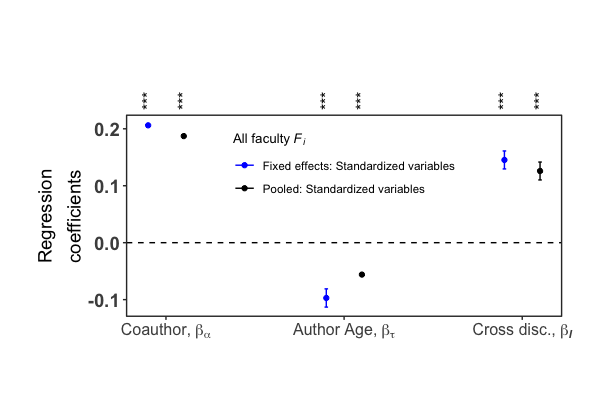
\includegraphics[width=9.3cm, height=7cm]{5A.png}
  \endminipage\hfill
  \minipage{0.5\textwidth}%
    \textbf{B}\\
    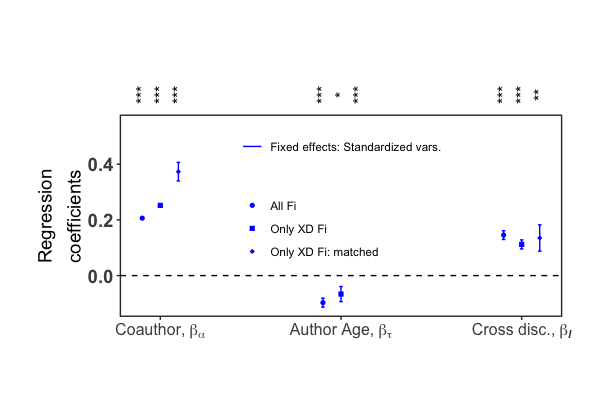
\includegraphics[width=9.3cm, height=7cm]{5B.png}
  \endminipage\hfill
  \minipage{0.5\textwidth}
    \textbf{C}\\
    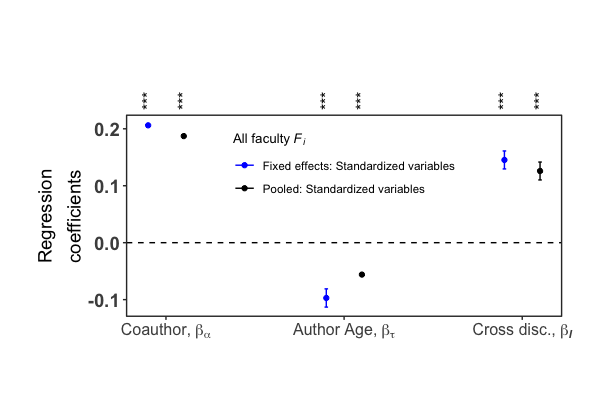
\includegraphics[width=9.3cm, height=7cm]{5A.png}
  \endminipage\hfill
  \minipage{0.5\textwidth}%
    \textbf{D}\\
    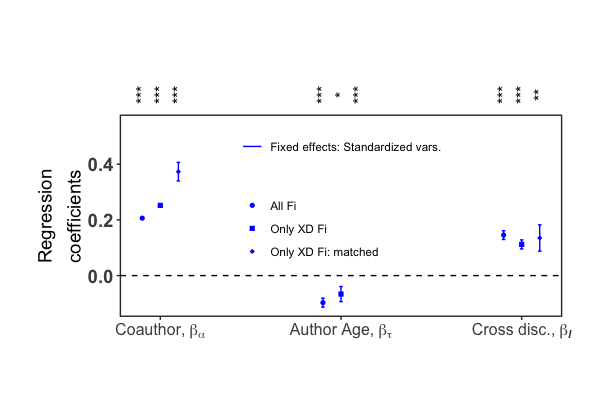
\includegraphics[width=9.3cm, height=7cm]{5B.png}
  \endminipage
  \caption{Career panel regression model}
  \label{fig:5}
\end{figure}

Figure 5A displays model estimates for Coauthors, Author age and Crossdisciplinarity. Interestingly for the purposes of this project, there is a significant effect of crossdisciplinarity on citation impact. Thus, it can be concluded that cross disciplinary papers are more heavily cited than biology or computer science genomics papers and therefore crossdisciplinarity positively effects the impact which publications make on the body of knowledge in the field of genomics. Significant effects for Co-authorship and Author age are also observed. The differences between fixed effects models and pooled models appear to be minimal, with similar significant relationships being observed in each case regardless of fixed effects. Figure 5B also examines the relationships of Coauthors, Author age and Crossdisciplinarity on citation impact, with fixed effects models being compared across different subsets of the overall data set. The figure compares all $F_i$, all XD $F_i$, and the pair matched subset of 53 matched $F_i$. Significant effects of all three characteristics are observed for each of the three $F_i$ subsets. It certainly makes sense that the more coauthors a paper has, the greater the citation impact would be. Large research teams tend to attract more attention than small ones in many fields. The important relationship between crossdisciplinarity and citation impact remains in all three $F_i$ subsets as well, demonstrating that the robust model is able to demonstrate that cross disciplinary publications are more likely to make a large impact in the literature when compared to biology or computer science genomics papers. Figure 5C displays the probability distribution for the placebo model in order to test for effects greater than the set Cross-disciplinarity coefficient shown in the blue dashed line. This shows that it is not down to chance that cross disciplinary papers made a greater impact in the literature than single-discipline papers in genomics. Figure 5D repeats the result displayed in Figure 5C, with the difference being that only XD $F_i$ are included in the experiment. Once again, a similar result is observed, no value within the cross-disciplinarity probability distribution is as large as the set coefficient. This further confirms the overarching result of this paper, that cross-disciplinarity is related to and directly impacts the citation impact which a paper makes in the genomic literature. 

\newpage
\section{Supplementary Table S4}
% !Rnw root = ../ProjectReport.Rnw
\begin{table}[H]
\begin{tabular}{m{5cm} m{3.0cm} m{3cm} m{2.5cm} m{2.7cm}}
\hline
\hline
& \textbf{No Fixed Effects} & \textbf{No Fixed Effects [Standardized]} & \textbf{Fixed Effects} & \textbf{Fixed Effects [Standardized]} \\ \hline
\multicolumn{5}{l}{\textbf{Publication characteristics}} \\
\rowcolor{lightgray}
{\# of author, $\beta_\alpha$} & 0.2836*** & 0.1872*** & 0.312*** & 0.2061*** \\
                             & (0.0025) & (0.0016) & (0.00262) & (0.00173) \\
\rowcolor{lightgray}
{Career age, $\beta_\tau$} & -0.00547*** & -0.0560*** & -0.00949*** & -0.0971*** \\
                         & (0.0002) & (0.0018) & (0.00156) & (0.01601) \\
\rowcolor{lightgray}
{Cross-disciplinary indicator, $\beta_I$} & 0.1259*** & 0.1259*** & 0.1453*** & 0.1453*** \\
                                        & (0.0157) & (0.0157) & (0.01578) & (0.01578) \\ \hline
\multicolumn{5}{l}{\textbf{Network characteristics}} \\
\rowcolor{lightgray}
{Author centrality, $\beta_\zeta$} & 0.0440*** & 0.0284*** & X & X \\
                             & (0.0029) & (0.0018) &  &  \\
\rowcolor{lightgray}
{Bridge ratio, $\beta_\lambda$} & 0.3338*** & 0.1210*** & X & X \\
                             & (0.0055) & (0.0020) &  &  \\
\rowcolor{lightgray}
{Discipline ($F$) dummy}     & 0.00790* & 0.0079* & X & X \\
                             & (0.0033) & (0.0033) & &  \\
\rowcolor{lightgray}
{Constant}                 & 0.4586*** & 0.1638* & -0.2932*** & -0.0669** \\
                         & (0.0761) & (0.0728) & (0.0456) & (0.0176) \\
\rowcolor{lightgray}
{Year dummy}            & Y & Y & Y & Y \\ \hline
\rowcolor{lightgray}
{n}                      & 413,565 & 413,565 & 413,565 & 413,565 \\
\rowcolor{lightgray}
{adj. $R^2$}             & 0.055 & 0.055 & 0.036 & 0.036 \\ \hline \hline
\multicolumn{5}{l}{\footnotesize{Standard errors in parentheses below estimate * p $\leq$ 0.05, ** p $\leq$ 0.01, *** p $\leq$ 0.0001}}

\end{tabular}
\caption{Career data set: Panel model on all falcuty}
\label{tbl:sT5}
\end{table}

All faculty $F$ were included in the panel model. Columns included in the table are divided by the inclusion of fixed effects, with no fixed effects included in the first two columns and fixed effects included in the following two. The second and fourth columns are standardized using the effect of a one standard deviation shift in the independent variable on the dependent variable. Although all faculty were meant to be included in the model, n = 3900 due to the inclusion of $F_i$ who have defined page rank centrality within the data set. All relevant publication characteristics and network characteristics are shown to have a significant effect of the scholarly impact which publications within the data set have. In fact, all characteristics within the table can be considered highly significant due to a p-value of less than or equal to 0.001.   

\newpage
\section{Supplementary Table S5}
% !Rnw root = ../ProjectReport.Rnw
\begin{table}[H]
\begin{tabular}{m{5cm} m{3.0cm} m{3cm} m{2.5cm} m{2.7cm}}
\hline
\hline
& \textbf{No Fixed Effects} & \textbf{No Fixed Effects [Standardized]} & \textbf{Fixed Effects} & \textbf{Fixed Effects [Standardized]} \\ \hline
\multicolumn{5}{l}{\textbf{Publication characteristics}} \\
\rowcolor{lightgray}
{\# of author, $\beta_\alpha$} & 0.329***  & 0.236*** & 0.351*** & 0.252*** \\
                             & (0.0037) & (0.0027) & (0.00392) & (0.00282) \\
\rowcolor{lightgray}
{Career age, $\beta_\tau$} & -0.00499*** & -0.0536*** & -0.00617* & -0.0663* \\
                         & (0.0003) & (0.0030) & (0.00253) & (0.0271) \\
\rowcolor{lightgray}
{Cross-disciplinary indicator, $\beta_I$} & 0.1095*** & 0.1095*** &  0.112*** & 0.112*** \\
                                        & (0.0165) & (0.0165) & (0.0162) & (0.0162) \\ \hline
\multicolumn{5}{l}{\textbf{Network characteristics}} \\
\rowcolor{lightgray}
{Author centrality, $\beta_\zeta$} & 0.0526*** & 0.0333*** & X & X \\
                             & (0.0046) & (0.0029) &  &  \\
\rowcolor{lightgray}
{Bridge ratio, $\beta_\lambda$} & 0.3192*** & 0.1116*** & X & X \\
                             & (0.0092) & (0.0032) & & \\
\rowcolor{lightgray}
{Discipline ($F$) dummy}     & -0.0383*** & -0.0383*** & X & X \\
                             & (0.0052) & (0.0052) & & \\
\rowcolor{lightgray}
{Constant}                 & 0.2113 & -0.0287 & -0.408*** & -0.0370* \\
                         & (0.1236) & (0.1187) & (0.0778) & (0.0285) \\
\rowcolor{lightgray}
{Year dummy}            & Y & Y & Y & Y \\ \hline
\rowcolor{lightgray}
{n}                      & 166,621 & 166,621 & 166,621 & 166,621 \\
\rowcolor{lightgray}
{adj. $R^2$}             & 0.067 & 0.067 & 0.049 & 0.049 \\ \hline \hline
\multicolumn{5}{l}{\footnotesize{Standard errors in parentheses below estimate * p $\leq$ 0.05, ** p $\leq$ 0.01, *** p $\leq$ 0.0001}}

\end{tabular}
\caption{Career data set: Panel model on all $XD_F$ falcuty}
\label{tbl:sT5x}
\end{table}

In order to conduct a robustness check for the panel model, all $F_i$  with XD orientation (n = 1247) were included. The stricter inclusion criteria for this model appears to have impacted the effect of the characteristics included in the panel model when compared to the results in Table S4. Although all characteristics still appear to have a significant impact on the impact which researchers in the data set have on the body of genomics literature, some of these effects appear to be diminished in the new model. The p-values associated with the different models for Career age and Author centrality are no longer less than or equal to 0.001. This perhaps means that the impact of XD publications on the literature is not as dependent on these two characteristics. 

\newpage
\section{Supplementary Table S6}
% !Rnw root = ../ProjectReport.Rnw
\begin{table}[H]
\begin{tabular}{m{5cm} m{3.0cm} m{3cm} m{2.5cm} m{2.7cm}}
\hline
\hline
& \textbf{No Fixed Effects} & \textbf{No Fixed Effects [Standardized]} & \textbf{Fixed Effects} & \textbf{Fixed Effects [Standardized]} \\ \hline
\multicolumn{5}{l}{\textbf{Publication characteristics}} \\
\rowcolor{lightgray}
{\# of author, $\beta_\alpha$} & 0.329***  & 0.236*** & 0.351*** & 0.252*** \\
                             & (0.0037) & (0.0027) & (0.00392) & (0.00282) \\
\rowcolor{lightgray}
{Career age, $\beta_\tau$} & -0.00499*** & -0.0536*** & -0.00617* & -0.0663* \\
                         & (0.0003) & (0.0030) & (0.00253) & (0.0271) \\
\rowcolor{lightgray}
{Cross-disciplinary indicator, $\beta_I$} & 0.1095*** & 0.1095*** &  0.112*** & 0.112*** \\
                                        & (0.0165) & (0.0165) & (0.0162) & (0.0162) \\ \hline
\multicolumn{5}{l}{\textbf{Network characteristics}} \\
\rowcolor{lightgray}
{Author centrality, $\beta_\zeta$} & 0.0526*** & 0.0333*** & X & X \\
                             & (0.0046) & (0.0029) &  &  \\
\rowcolor{lightgray}
{Bridge ratio, $\beta_\lambda$} & 0.3192*** & 0.1116*** & X & X \\
                             & (0.0092) & (0.0032) & & \\
\rowcolor{lightgray}
{Discipline ($F$) dummy}     & -0.0383*** & -0.0383*** & X & X \\
                             & (0.0052) & (0.0052) & & \\
\rowcolor{lightgray}
{Constant}                 & 0.2113 & -0.0287 & -0.408*** & -0.0370* \\
                         & (0.1236) & (0.1187) & (0.0778) & (0.0285) \\
\rowcolor{lightgray}
{Year dummy}            & Y & Y & Y & Y \\ \hline
\rowcolor{lightgray}
{n}                      & 166,621 & 166,621 & 166,621 & 166,621 \\
\rowcolor{lightgray}
{adj. $R^2$}             & 0.067 & 0.067 & 0.049 & 0.049 \\ \hline \hline
\multicolumn{5}{l}{\footnotesize{Standard errors in parentheses below estimate * p $\leq$ 0.05, ** p $\leq$ 0.01, *** p $\leq$ 0.0001}}

\end{tabular}
\caption{Career data set: Panel model on all $XD_F$ falcuty: matching}
\label{tbl:sT6}
\end{table}

This table contains the results of a panel model robustness check with and without fixed effects. In order to perform the robustness check, $F_i$ were selected for inclusion based on matched pairs. Criteria for matched pairs included the matching of an XD publication to a non-XD publication which were published within two years of each other, with within 20\% similar number of coauthors. $F_i$  included in the model (n = 53) had at least 10 such matched pairs. Using the matching process, a counterfactual was able to be properly defined for each XD publication. Thus, underlying connections between XD publications and greater impact on the body of literature could be explored. Similar to the comparison between Tables S4 and S5, with the even stricter criteria for inclusion in the model for Table S6 the effect of certain characteristics within the model on a publication’s scholarly impact changes in this model. The number of coauthors which a publication has remains strongly related to scholarly impact with a p-values of less than or equal to 0.001. There is no significant effect of career age observed for the model without fixed effects, whereas career age with fixed effects remains highly significant. The significant effects of author centrality and bridge fraction remain, although they are only significant to alpha levels of 0.05 and 0.01, respectively. As the data set is more and more limited, most of the significant effects remain with regards to the impact which publications make on the body of knowledge in genomics.

\bigskip   % leave some empty space (optional)

\end{document}

